% Esto es un magic comment para indicar el compilador. En este caso es XeLaTeX.
%%& --job-name=mypdf
%%& --quiet
% !TeX program = lualatex
% !TeX spellcheck = es_ES
% !TeX encoding = utf8

\documentclass{article}
\usepackage{enumitem}
\setlistdepth{5}
%\usepackage[utf8]{inputenc}
%%%%%%%%%%%%%%%%%%%%%
%%%%%% FONTS
%%%%%%%%%%%%%%%%%%%%%
\usepackage{fontspec}
\usepackage[T1]{fontenc}
\DeclareTextFontCommand{\textcmcsans}{\cmcsans}
\newfontfamily\cmcsans{Comic Sans MS}


\newcommand{\rmfont}[1]{{\fontfamily{ptm}\selectfont%
#1}}
\newcommand{\rmfontbf}[1]{{\fontfamily{ptm}\selectfont%
\textbf{#1}}}
\newcommand{\rmfontsc}[1]{{\fontfamily{ptm}\selectfont%
\textsc{#1}}}
\newcommand{\vbfont}[1]{{\fontfamily{lmtt}\selectfont%
#1}}
\newcommand{\vbfontbf}[1]{{\fontfamily{lmtt}\selectfont%
\textbf{#1}}}
\newcommand{\lazyfox}{The quick brown fox jumps over the sleazy dog}
\newcommand{\dofont}[1]{\fontfamily{#1}\selectfont \lazyfox}
%% ------------------------- FONT
\usepackage[spanish,mexico
]{babel}
    \usepackage[utopia]{mathdesign}

\usepackage[a4paper,left=3cm,right=3cm,top=2cm,bottom=2cm]{geometry}
\usepackage{graphicx,xcolor,pdfpages,caption,subcaption,soul,fontawesome,wrapfig}
%BIBLIO
\usepackage{natbib}

% FANCY
\usepackage{fancyhdr}
\fancypagestyle{regular}{
\fancyhf{}
\setlength{\headheight}{15.2pt}
\pagestyle{fancy}
\lhead{\LaTeX{} para principiantes}
\rhead{Patricio Whittingslow}
\cfoot{\thepage}
}

\fancypagestyle{codeExample}{
\setlength{\headheight}{15.2pt}
\pagestyle{fancy}
\lhead{\LaTeX{} para principiantes}
\chead{Resultado del código \ref{cod:documentheader}}
\rhead{Patricio Whittingslow\\ Fulano de Tal}
\cfoot{\thepage}
}

% \setlength{\headheight}{15.2pt}
% \pagestyle{fancy}
% \lhead{\LaTeX{} para principiantes}
% \rhead{Patricio Whittingslow}
% \cfoot{\thepage}
\usepackage[urlcolor=blue,colorlinks=true,
citecolor=red]{hyperref}
\usepackage{mdframed,cancel,amsmath}




\newmdtheoremenv[%
linecolor=gray,
leftmargin=30,%
rightmargin=0,
backgroundcolor=blue!4,%
innertopmargin=2pt,%
ntheorem]{code}{Código}[section]

\newmdtheoremenv[%
linecolor=gray,
leftmargin=30,%
rightmargin=0,
backgroundcolor=red!4,%
innertopmargin=2pt,%
ntheorem]{code2}{Código}[section]
\newmdtheoremenv[%
linecolor=gray,
leftmargin=30,%
rightmargin=0,
backgroundcolor=green!4,%
innertopmargin=2pt,%
ntheorem]{code3}{Código}[section]
% \usepackage{standalone}
\title{\Huge \bf \LaTeX{} para principiantes \\ {\LARGE con ejemplos}}
\author{Patricio Whittingslow}
\date{\today}


% \newcommand{\symbentry}[2]{$#1$& #1 &#2}
\newcommand{\tbs}{\textbackslash}
\newcommand{\textbi}[1]{\textbf{\textit{#1}}}
\newcommand\numberthis{\addtocounter{equation}{1}\tag{\theequation}}



\begin{document}
{\centering
{\bf \Huge \LaTeX{} para principiantes \par}
\vspace{.2cm}
{\bf \LARGE con ejemplos \par}
\vspace{.5cm}
{\large Patricio Whittingslow\par}
\vspace{.3cm}
{\large \today \par}
}

\tableofcontents
\vspace*{\fill}
 \begingroup

\fontfamily{pbk}\selectfont
\noindent
 Licencia: \faCreativeCommons~BY-NC-SA 4.0
 
  Versión Preliminar 2
 \endgroup
 
\clearpage
\pagestyle{regular}
\section{Introducción}
La idea es compilar información que sea útil tener a mano cuando se programa en \LaTeX. Si el lector es nuevo al \LaTeX{} y quiere empezar a programar \emph{ya} se puede referir al código \ref{cod:firstblood} que es un ejemplo simple como para ir agarrándole la mano.\footnote{Se recomienda usar el compilador online \href{https://www.overleaf.com}{Overleaf} (\href{https://www.overleaf.com}{link})} El \LaTeX{} es un lenguaje compilado,\footnote{\LaTeX{} además es \href{https://stackoverflow.com/qu estions/2968411/ive-heard-that-latex-is-turing-complete-are-there-any-programs-written-in-late}{Turing complete}!} por lo cual se va tener que compilar su archivo \verb|.tex| cada vez que quiera ver como va quedando.

\begin{code}\label{cod:firstblood}
\begin{verbatim}

\documentclass{article}
\begin{document} 
Mi documento empieza aqui! Puedo crear secciones:
\section{La primera seccion}
El \LaTeX{} es demasiado facil de usar, pero cuesta amaestrarlo.
\end{document}
\end{verbatim}
\end{code}
a medida que vaya desarrollando el documento, tal vez se encuentre con limitaciones. El código \ref{cod:firstblood} como está no acepta tildes. Esto se arregla agregando paquetes al preámbulo. Para usar tildes veremos con agregar la linea \verb|\usepackage[utf8]{inputenc}| alcanza y sobra.
\section{El Preámbulo}


El preámbulo es el código que va antes del documento en si. Contiene los paquetes que uno usa en el código, sea la fuente, el tamaño de letra, etc. 

Lista corta de cosas que el preámbulo puede modificar
\begin{itemize}
    \item Estilo de fuente: tamaño, tipo
    \item \verb|graphicx| para agregar fotos y gráficos
    \item Geometría de la pagina con paquete \verb|geometry|
    \item ``Renovación" de comandos, y creación de comandos nuevos.
    \item Paquetes de matemática y escritura como \verb|amsmath|, \verb|siunitx| (Sistema Internacional) y \verb|soul|
    \item Mas paquetes de lo que podes imaginarte como \verb|movie| (animaciones),  \verb|tikz| \href{http://www.texample.net/tikz/examples/}{(tipo, wow.),} etc y etc.
\end{itemize}
\subsection*{Típico preámbulo}
En verdad alcanza con solo tener \verb|\documentclass{article}| en el preámbulo, pero esto no te va llevar muy lejos. Siempre es bueno aprovechar de los paquetes que tiene para ofrecer el \LaTeX! 
\begin{code}
\begin{verbatim}

\documentclass[12pt, titlepage]{article} %Esto es un comentario!
\usepackage[spanish]{babel} %Español
\usepackage[utf8]{inputenc} %Para mis tildes
\usepackage{graphicx} % Para mostrar gráficos
\usepackage{enumitem} % Paquetes varios
%Se pueden agregar paquetes diferentes separando con coma:
\usepackage{soul,cancel}
\usepackage{gensymb} %Esté es el preámbulo de un TP de termodinámica
\usepackage{siunitx} %El compilador no lee los comentarios
\end{verbatim}
\end{code}



Verán que le suele preceder un texto entre corchetes al paquete (o clase de documento). Estos son los parámetros o \emph{opciones} del paquete. La mayoría de las veces no hace falta meter opciones aunque algunos paquetes lo requieren, como \verb|babel| que necesita el input \verb|[spanish]| para saber que castellano es el idioma seleccionado entre tantos otros.

\subsection*{Clase de documento}
Todo documento común y corriente de \LaTeX{} empieza eligiendo la clase de documento. Se tienen las siguientes para elegir
\begin{itemize}
    \item \verb|article| El típico informe corto, artículos cientificos...
    \item \verb|beamer| Para presentaciones del estilo powerpoint
    \item \verb|report| Para informes muy largos con varios capítulos o para una tesis
    \item \verb|book| Para escribir libros
    \item \verb|proc| Procedimientos
    \item \verb|memoir| igual a la \verb|book| pero mas flexible
    \item \verb|slides| Literalmente, filminas
    \item \verb|letter| Para escribir cartas
    \item \verb|IEEEtrans| Para artículos con formato de la revista \emph{Transactions} de la IEEE
\end{itemize}
donde cada uno tiene sus opciones y sus manías. En esté documento se va tratar solamente el tipo \verb|article|.

\textbf{Opciones para } \verb|article|:
\begin{itemize}
    \item \verb|xpt| donde \verb|x| es el tamaño de la fuente
    \item \verb|abstract|
    \item \verb|titlepage| Agrega posibilidad de hacer una portada
\end{itemize}
\section{Escritura básica de documento} \label{sec:EntornoDocument}
Lo que aparece en el documento es lo que está en el \textbi{entorno}  \verb|document|. Con entorno me refiero a todo lo que está en las lineas entre \verb|\begin{document}| (en inglés: $\backslash$Comenzar$\{$documento$\}$) y \verb|\end{document}| ($\backslash$Terminar$\{$documento$\}$). Esto se puede apreciar mejor en el código \ref{cod:entornoDocument}.
\begin{code} \label{cod:entornoDocument}
\begin{verbatim}

%Acá va el preámbulo
\begin{document} %Aca empieza el entorno document
Mi primer documento LaTeX. 

%El entorno documento acaba en está linea
\end{document}
Todo lo que esta acá afuera no lo lee el compilador!
\end{verbatim}
\end{code}
naturalmente, queremos que lo que escribamos aparezca en el archivo \verb|.pdf| de salida, por lo tanto escriban \emph{dentro} del entorno \verb|document|! Para continuar, abra un archivo y vaya probando los siguientes comandos, y si piensa poner tildes, no se olvide de agregar el paquete en su preámbulo:

\noindent\verb|\usepackage[utf8]{inputenc}| !

\subsection{Secciones e índice}
Para agregar una sección se usa el comando \verb|\section{Nombre-de-mi-Sección}|. Después de agregar una sección podes empezar a escribir directamente abajo. También existen \verb|\subsection| y \verb|\subsubsection| usados de la misma forma. Se suele recomendar no numerar las subsecciones, aunque es un tema de gusto personal. Esto se logra mediante el operador asterisco \verb|*|. Por ejemplo,\linebreak
\verb|\subsection*{Sección No Numerada}|. Las secciones no numeradas \textbf{no} aparecen en el Índice\linebreak (\verb|\tableofcontents|).

Una vez que se tenga muchas secciones, subsecciones, etc... se justifica el uso de un índice. El índice suele ser puesto antes de la primera sección y después del resumen (\emph{abstract}) con el comando:\linebreak \verb|\tableofcontents|.

\subsection{Título}
Lo segundo mas importante después del contenido es tener un título. Hay varias formas de agregarle un titulo a un documento. La mas sencilla es dejar que \LaTeX{} te lo haga. En el preámbulo\footnote{No es necesario agregarlo en el preámbulo, pero es lo más prolijo.} podes agregar el nombre de la obra con \verb|\title|, el autor con \verb|\author| y la fecha \verb|\date|.
\begin{code}\label{cod:SimpleTitle}
\begin{verbatim}

\title{Como crecer hongos en casa}
\author{Pato \\ Fulano}
\date{\today}
\thanks{Mom}
\begin{document}
\maketitle
Como queda?
\end{document}
\end{verbatim}
\end{code}

\textbf{Author.} Pausemos un segundo. Que hacen esas dos barritas? Pues, nos permiten escribir nombres de autores en diferentes lineas. Basta con decir que no son necesarias pero pueden resultar útiles. 

\textbf{Date.} Puede ser que el comando \verb|\today| nos llame la atención. No suele ser el caso que un comando tome otro comando como argumento, en esté caso nos aseguramos que \verb|\date| imprima el día completo. Si no se quiere el día se puede optar por el comando \verb|\date{}|. Otro ejemplo:\linebreak \verb|\date{1 de enero 1970}|.

\subsection{Carátula}
\emph{La carátula probablemente es el lugar donde uno mejor puede desatar su creatividad cuando programa en} \LaTeX. 

En el caso que uno no sea fan de la movida creativa puede agregar la opción \textit{titlepage} con

\noindent\verb|\documentclass[titlepage]{article}| al código \ref{cod:SimpleTitle}. Con dicho cambio se obtiene una carátula mínima no-editable.

Si uno quiere diseñar una carátula se puede volver loco con la cantidad de posibilidades. A continuación tiene un ejemplo usando el entorno \verb|titlepage| y el resultado:\footnote{Se invita al lector buscar ``Modelo de un Informe Técnico ITBA'' en los \emph{templates} disponibles en Overleaf.}
\clearpage

\begin{code} \label{cod:TituloTecnico}
\begin{verbatim}

\documentclass[10pt,titlepage]{article}
\usepackage[a4paper,
            top=2.5cm,
            bottom=2cm,
            left=3cm,
            right=3cm,
            marginparwidth=1.75cm,
            headheight=28pt]{geometry}
\usepackage[utf8]{inputenc}
\usepackage[scaled=1]{helvet}
\usepackage[format=plain,
            labelfont={bf,it},
            textfont=it]{caption}
\renewcommand{\familydefault}{\sfdefault}
\usepackage{graphicx}
\begin{titlepage}
\centering
{ \large Instituto Tecnológico de Buenos Aires  \par }
\vspace{2cm}
{\Large \scshape Mecánica de Fluidos - 31.26 \par}
\vspace{2cm}
{\Huge \scshape  Trabajo Practico \par }
\vspace{1cm}
{\large \bf Grupo 10 \par}
\vspace{0cm}
\textsc{\large Fulano -- 56175 \\ Mengano -- 56388 \\
Zotano -- 54289 \\ Patano -- 55423}
\vspace{2cm}
{\par \large Fecha de mediciones: 7 de junio de 2018 \par}
\vspace{1cm}
{\large Fecha de entrega: 19 de junio de 2018\par}
\vspace{2.5cm}
{\large Comentarios: .......................................}\\
\vspace{1.2cm}
{\large ............................
..................................}
\vspace{1cm}
\begin{figure}[htb!]
\centering

\includegraphics[width=6cm]{fig/logoitba.png}
\end{figure}
\end{titlepage}
\end{verbatim}
\end{code}
\clearpage
%%%%%%%%%%%%%%%%%%%%
%% TITLE PAGE
%%%%%%%%%%%%%%%%%%%%



\includepdf{pdf/caratula.pdf}


% \pagenumbering{arabic}
% \setcounter{page}{6}

\subsection{Encabezado, pie de página y notas a pie de página}\vspace{-.1cm}
El encabezado se entiende como el conjunto de textos que se inscribe en la parte superior de las páginas de un documento. Puede llegar a incluir el nombre del autor, el título del trabajo, o la fecha. El pie de página se encuentra en la zona inferior y suele tener el número de página, como en este caso.

Con agregar el siguiente código a un documento se puede obtener un encabezado simple y aburrido.
\begin{code}
\begin{verbatim}
    
\pagestyle{myheadings}
\markright{Mi Documento \hfill Mi nombre \hfill}
\end{verbatim}
\end{code}

{\bf No fun. }El resultado no dice mucho. No se tiene buen control sobre la posición del número de página y si el texto es muy largo puede entrar en interferencia con el número de página.\par

{\tt \bf Hfill}. Junto con su hermano \verb|\vspace*{\fill}|, son opciones muy útiles para llenar espacio y formatear cualquier número de objetos que uno se pueda imaginar.

A continuación: usando el paquete \vbfont{fancyhdr} se pueden obtener unos resultado fantásticos\footnote{Si se va usar en conjunto con \vbfont{geometry} declarar este ultimo primero!}
\begin{code}\label{cod:documentheader}
\begin{verbatim}

\usepackage{fancyhdr}
\setlength{\headheight}{15.2pt}
\pagestyle{fancy}
\lhead{\LaTeX{} para principiantes}
\rhead{Patricio Whittingslow \\ Fulano de Tal}
\cfoot{\thepage}
\end{verbatim}
\end{code}
\pagestyle{codeExample}

{\bf Resultados.} El resultado de este código se puede apreciar en el encabezado de este mismo documento! Mire! $\uparrow$

{\bf Lhead.} Los comandos para editar el encabezado y pie son
\begin{itemize}
    \item \verb|\lhead|
    \item \verb|\chead|
    \item \verb|\rhead|
    \item \verb|\lfoot|
    \item \verb|\cfoot|
    \item \verb|\rfoot|
\end{itemize}
los cuales corresponden al encabezado, \emph{head} y al pie, \emph{foot}. La letra que precede (\vbfont{l,c,r}: \emph{left, center, right}) corresponde a izquierda, centro y derecha, respectivamente. Por defecto \vbfont{fancyhdr} te viene con el número de página en el pie centrado y con secciones numeradas en el encabezado a la derecha.

{\bf Continuación de lectura.} Si uno tiene un interés especial por encabezados puede continuar su lectura en \href{https://en.wikibooks.org/wiki/LaTeX/Customizing_Page_Headers_and_Footers}{wikibooks}.

{\bf Nota al pie de página.} Sí uno quiere hacer una acotación al pie de página puede usando el comando \vbfont{footnote}.
\begin{code}\label{cod:footnote}
\begin{verbatim}

Si tengo que aclarar algo que no es esencial al texto,
haré lo más responsable.\footnote{Ponerlo al pie de página.}
\end{verbatim}
\end{code}
Resultado del código \ref{cod:footnote}:

\begin{mdframed}
Si tengo que aclarar algo que no es esencial al texto, haré lo más responsable.\footnote{Ponerlo al pie de la página.}
\end{mdframed}

\subsection{Geometría de página y formateo general}
Se refiere a todo lo que sea ajustes de tamaño de página, margenes y formateo de texto. El paquete \vbfont{geometry} es fundamental para cualquier documento. Permite economizar espacio de la página y seleccionar el tamaño \vbfont{a4paper} para los que no imprimimos con páginas \vbfont{letter} (seleccionado por defecto). El paquete \vbfont{geometry} es muy amplio y se puede hacer \href{http://texdoc.net/texmf-dist/doc/latex/geometry/geometry.pdf}{cualquier} cantidad de acrobacias con el. 

\begin{code}\label{cod:geometryBasic}
\begin{verbatim}

\usepackage[a4paper,
            left=3cm,
            right=3cm,
            top=2cm,
            bottom=2cm]{geometry}
\end{verbatim}
\end{code}

\textbf{Margenes.} Con las opciones del código \ref{cod:geometryBasic} el texto va estar contenido en un cuadro\footnote{Cabe destacar que es un cuadro ``virtual", solo el compilador se entera que existe.} con sus bordes laterales a 3 centímetros del borde de la hoja y a 2 centímetros de los bordes superiores e inferiores.

Para formatear el espacio entrelineado, conocido en MS Word como \emph{line-spacing} ($L_s$) se suele usar el paquete \vbfont{setspace}, el cual cae lejos de ser un ejemplo de la elegancia del \LaTeX{}.

\begin{code} \label{cod:setspace}
\begin{verbatim}

\usepackage{setspace}
\linespread{X} 
\end{verbatim}
\end{code}
\pagestyle{regular}
\textbf{Halle} $X${\bf.} A seguir se tiene una expresión que {\bf no} es un resultado de un código, es la ecuación para obtener $X$ a partir del espacio-entrelineado deseado ($L_s$)

\[ X=\frac{5}{3}\cdot L_s - \frac{2}{3} \]

El comando \vbfont{linespread} toma un número (separador decimal punto) para espaciar las lineas de texto. Ejemplo: espaciado doble: $X=1.6$, espaciado medio: $X=1.3$, el famoso \emph{1.15 spacing} de MS Word:$X=1.25$

\textbf{Otros comandos del paquete}\vbfontbf{ setspace}. \verb|\singlespacing|,\verb|\onehalfspacing| y

\noindent\verb|\doublespacing|.


\subsection{Comandos}\label{sec:Comandos}
Los comandos ahorran tiempo y espacio en el código. Para familiarizarse, un pequeño ejemplo:
\begin{code}\label{cod:ejemploComando1}
\begin{verbatim}

% PREAMBULO ...
\newcommand{\superComando}{\noindent\textbf{Nota}$\rightarrow$}
\begin{document}
\superComando Jugo de mora, banana y frutilla

\superComando El \LaTeX{} tarda mucho en escribir
\end{document} %Lo podes usar cuantas veces quieras                            
\end{verbatim}
\end{code}
{Resultado del codigo \ref{cod:ejemploComando1}}:
\begin{mdframed}
\noindent\textbf{Nota}$\rightarrow$ Jugo de mora, banana y frutilla

\noindent\textbf{Nota}$\rightarrow$ El \LaTeX{} queda genial al compilar
\end{mdframed}

Con una pequeña modificación se puede agregar comandos que aceptan argumentos:
\clearpage
\begin{code}\label{cod:ejemploComando2}
\begin{verbatim}

% PREAMBULO ...
\newcommand{\ultraComando}[2]{$\frac{d#1}{d t}$ -- derivada 
de #2  respecto tiempo.}
\begin{document}
\ultraComando{x}{posicion}
\end{document} %Lo podes usar cuantas veces quieras                            
\end{verbatim}
\end{code}
Resultado del código \ref{cod:ejemploComando2}
\begin{mdframed}
$\frac{dx}{d t}$ -- derivada de posición respecto tiempo.
\end{mdframed}

\textbf{Argumentos}. El \verb|[2]| le indica al código cuantos argumentos toma el comando. El símbolo numeral seguido del número le indica donde va el input. 

Este ultimo código puede ahorrar muchísimo tiempo si se sabe donde emplear. La razón mas común por usar un comando es para representar algún valor, numero o notación que se suele repetir en el documento muy seguido, por ejemplo, derivadas parciales! Es mas corto hacerse un comando que tome dos valores, la variable a derivar y a que se deriva respecto de. Este comando tendría la forma de \verb|\newcommand{\dparcial}[2]{\frac{\partial #1}{\partial #2}}|. 
\section{Gráficos}
\subsection{Como agregar y ajustar una imagen}
Se pueden inscribir gráficos en el documento. Primero se tiene que agregar el archivo del gráfico a la carpeta de trabajo\footnote{En Overleaf uno está limitado a la carpeta de trabajo. Si uno trabaja con muchas fotos es conveniente usar un compilador ``\emph{offline}'' y de esa forma poder acceder todas las fotos en la computadora, sea donde estén. Se recomienda \textit{Kile} o \textit{MikTeX}.} y de ahí usar el paquete \verb|graphicx| y el siguiente código donde se quiere la imagen
\begin{code}\label{cod:CalvinHobbes}
\begin{verbatim}

\begin{figure}[htb!]
    \centering %Centra la imágen
    
\includegraphics[width=\textwidth]{calvinHobbes.jpg}}
    \caption{Subtitulo que explica la imagen. Es prescindible.}
    \label{fig:MiImagen}
\end{figure}
Como se puede ver en la figura \ref{fig:MiImagen}.
\end{verbatim}
\end{code}
\clearpage
\begin{mdframed}{Resultado del código \ref{cod:CalvinHobbes} \emph{Credito de imagen a Bill Waterson}}
{
    \centering %Centra la imágen
    
\includegraphics[width=\textwidth]{fig/calvinHobbes.jpg}
    \captionof{figure}{Subtitulo que explica la imagen. Es prescindible.}
    \label{fig:MiImagen}
}
Como se puede ver en la figura \ref{fig:MiImagen}.
\end{mdframed}

\textbf{Error.} Acordarse de agregar el paquete \verb|graphicx| y verificar que la imagen está en el directorio del archivo \verb|.tex| y que está bien escrito el nombre, minúsculas y mayúsculas donde van.

\textbf{Label y ref.} \LaTeX{} por si solo mantiene registro de las imágenes que se van usando y las numera. En cualquier momento puedo referir una imagen que haya usado en el texto, \verb|\ref{fig:MiImagen}|=\ref{fig:MiImagen}.

\textbf{Ancho/alto.} Se controla mediante los parámetros \verb|width| y \verb|height|. En este caso se uso el comando \verb|\textwidth| para que la figura tome el ancho del mismo texto. En lugar de \verb|\textwidth| se puede usar \verb|width=8cm| para obtener una imagen de ancho 8 centímetros.\footnote{Si se trabaja con columnas múltiples se recomienda al lector no confiar en estas unidades. Es mas, hasta que no se especifique el correcto tamaño de la pagina con el paquete \vbfont{geometry} las unidades especificadas no tendrán el aspecto correcto.} \LaTeX{} trabaja en las siguientes unidades:

\begin{itemize}
    \item \verb|mm| milimetros
    \item \verb|cm| centimetros
    \item \verb|in| pulgadas
    \item \verb|px| pixeles
    \item \verb|pt| points
\end{itemize}

\textbf{Float}\vbfontbf{[htb!].} 
\LaTeX{} es un programa orgulloso, cree que sabe exactamente donde poner cada imagen, o tabla, sin falta. Para los casos donde la pifie (casi siempre) se usa un \emph{float specifier}, una sugerencia por parte del usuario de donde poner la imagen. \verb|[h]| le sugiere al \LaTeX{} que la imagen vaya en el mismo lugar donde se encuentra en el código, \emph{here} (aquí). Se le pueden agregar segundos parámetros, en orden de prioridad. \verb|[tbh]| sugiere que vaya arriba de todo (\emph{top}), si no puede entonces abajo de todo (\emph{bottom}) y en el peor de los casos, pon la imagen donde está en el código (\emph{here}). Agregar un signo de exclamación convierte la sugerencia en una amenaza, de está forma se motiva más el \LaTeX{} en cumplir con el Float.
\subsection{Múltiples gráficos}
Al usuario le podrá interesar imprimir múltiples gráficos para ahorrar espacio para informes con longitud máxima o para vincular imágenes relacionadas con una etiqueta única.

A continuación hay un ejemplo usando los paquetes \vbfont{caption} y \vbfont{subcaption}.
\begin{code} \label{cod:multipleImages}
\begin{verbatim}

\begin{figure}[htb!]
\centering
\begin{subfigure}{.36\textwidth}
  \centering
  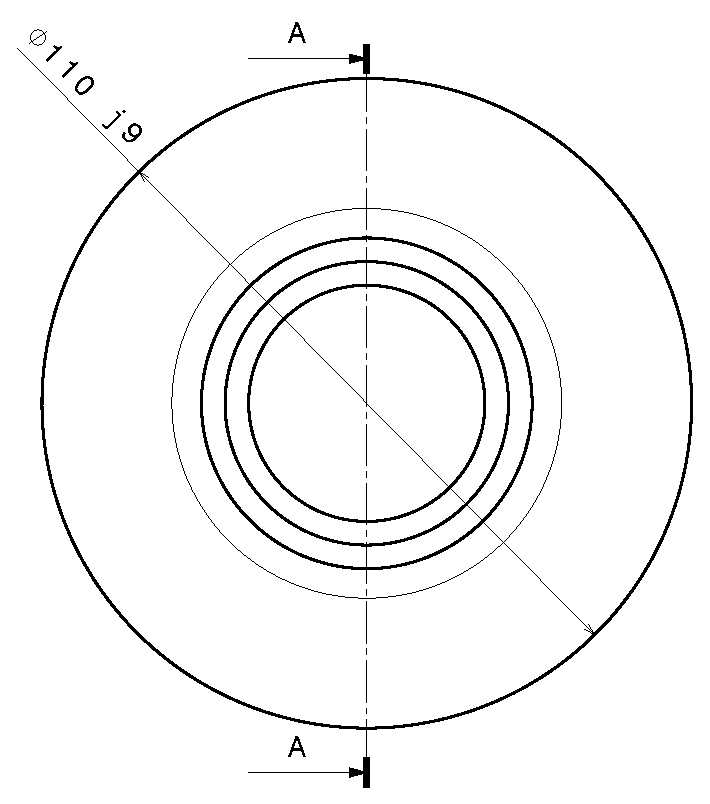
\includegraphics[height=4cm]{fig/toberaFrente.eps}
  \caption{Ver Norma PTC 19.5 - 2004.}
  \label{fig:tobFrente}
\end{subfigure}%
\begin{subfigure}{.33\textwidth}
  \centering
  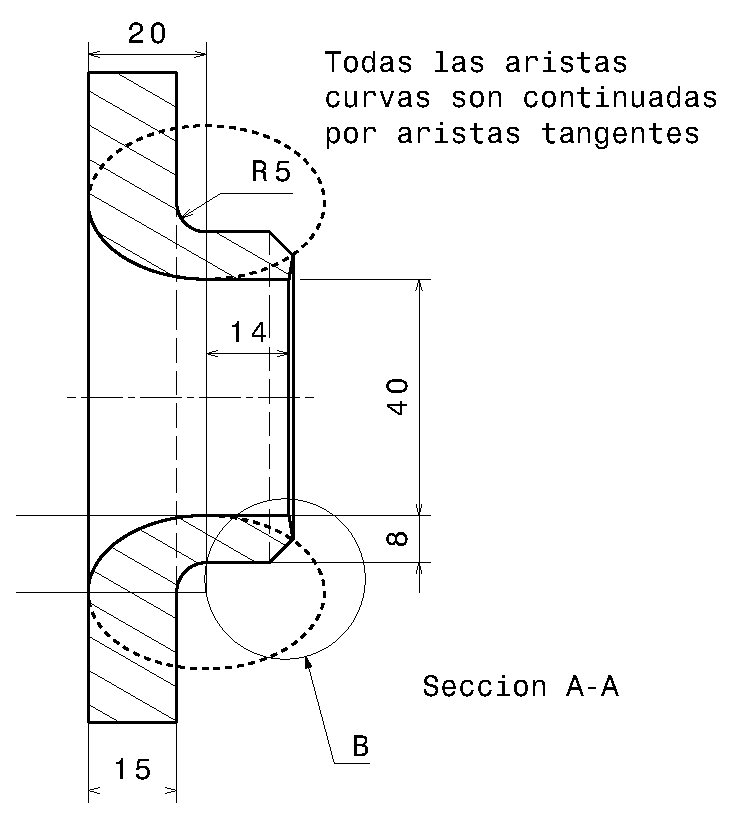
\includegraphics[height= 4cm]{fig/ToberaCorte.eps}
  \caption{Corte de Tobera.}
  \label{fig:tobSeccion}
\end{subfigure}
\begin{subfigure}{.27\textwidth}
  \centering
  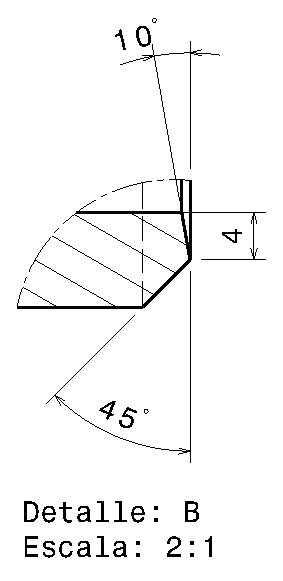
\includegraphics[height=4cm]{fig/ToberaDetalle.eps}
  \caption{Detalle de chaflán de tobera.}
  \label{fig:tobDetalle}
\end{subfigure}
\caption{Especificaciones para fabricación de tobera.}
\label{fig:tobConjunto}
\end{figure}
\end{verbatim}
\end{code}

Resultado del código \ref{cod:multipleImages}

\begin{figure}[htb!]
\begin{mdframed}
\centering
\begin{subfigure}{.36\textwidth}
  \centering
  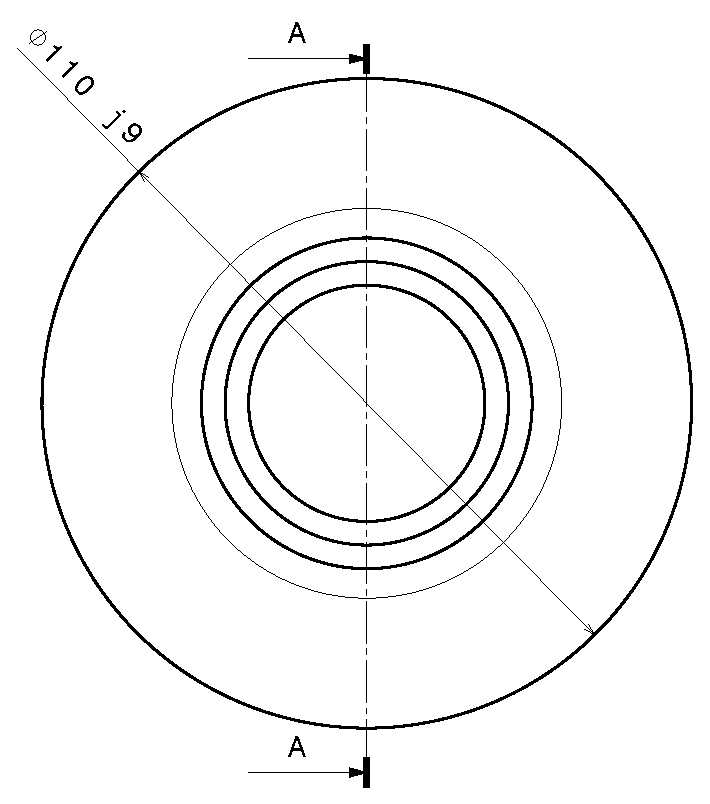
\includegraphics[height=4cm]{fig/toberaFrente.eps}
  \caption{Ver Norma PTC 19.5 - 2004.}
  \label{fig:tobFrente}
\end{subfigure}%
\begin{subfigure}{.33\textwidth}
  \centering
  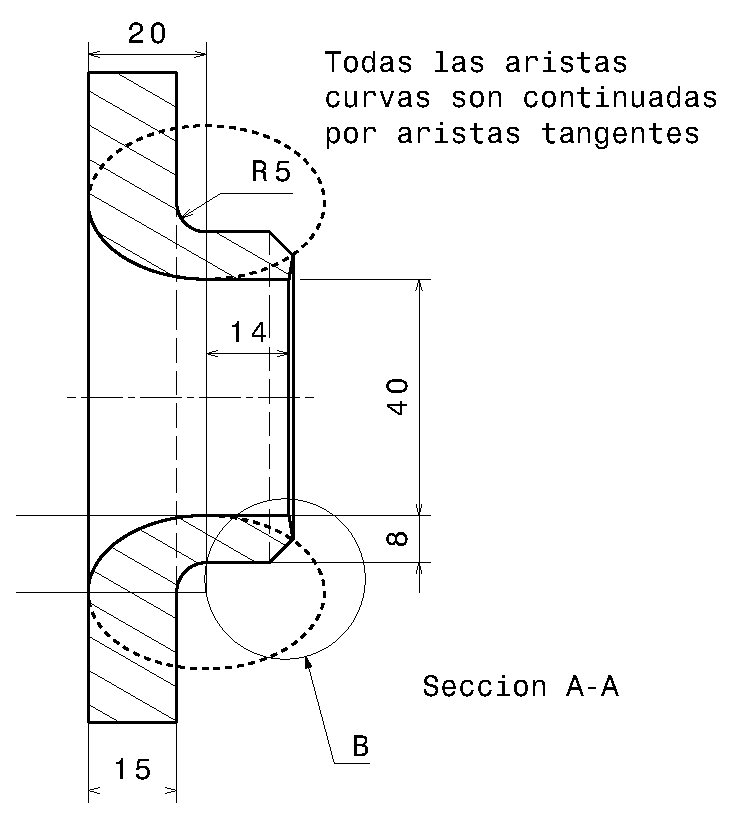
\includegraphics[height= 4cm]{fig/ToberaCorte.eps}
  \caption{Corte de Tobera.}
  \label{fig:tobSeccion}
\end{subfigure}
\begin{subfigure}{.27\textwidth}
  \centering
  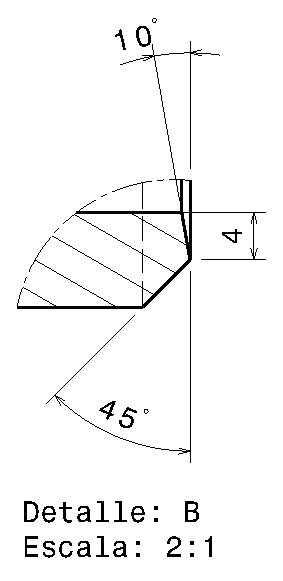
\includegraphics[height=4cm]{fig/ToberaDetalle.eps}
  \caption{Detalle de chaflán de tobera.}
  \label{fig:tobDetalle}
\end{subfigure}
\caption{Especificaciones para fabricación de tobera.}
\label{fig:tobConjunto}
\end{mdframed}
\end{figure}

\vbfontbf{subcaption.} Este formato incluso te permite referir subfiguras \verb|\ref{fig:tobSeccion}| \fbox{\ref{fig:tobSeccion}}  y el conjunto de figuras \verb|\ref{fig:tobConjunto}| \fbox{\ref{fig:tobConjunto}}.

\vbfontbf{subfigure.} Se puede controlar el espacio horizontal que ocupa cada figura declarando \verb|{X\textwidth}| con cada subfigura. La suma de las $X$ debería da menor a 1 si se las quiere todas en una fila. 
\subsection{Texto y gráficos entrelineados}
Un paquete excelente para ahorrar espacio en el documento es \vbfont{wrapfig}. Te permite tener una columna de texto con una figura al costado.
\clearpage  
\begin{code}\label{cod:wrapfig}
\begin{verbatim}

\begin{wrapfigure}{L}{0.5\textwidth}
    \includegraphics[width=7cm]{vigo.eps}
    \caption{Los archivos .eps son vectoriales.}
\end{wrapfigure}
Aquí iría tu texto. Se puede poner mucho texto
y no interfiere con la imagen. 
El paquete \verb|wrapfig| va como piña con imágenes esbeltas.
\end{verbatim}
\end{code}
Resultado del código \ref{cod:wrapfig}: 
\begin{mdframed}
\begin{wrapfigure}{L}{0.5\textwidth}
    \includegraphics[width=7cm]{fig/vigo.eps}
    \caption{Los archivos .eps son vectoriales.}
\end{wrapfigure}

Aquí iría tu texto. Se puede poner mucho texto y no interfiere con la imagen. El paquete \verb|wrapfig| va como piña con imágenes esbeltas.
\vspace{5.8cm}
\end{mdframed}

\vbfontbf{wrapfigure.} Se puede elegir el lado en el cual va la figura, en este ejemplo se eligió el lado izquierdo con el segundo parámetro \verb|{L}| (\emph{Left}). Usar \verb|{R}| para lado derecho.  También se tiene que indicar el limite al cual llega la imagen con el segundo parámetro. En este caso \verb|{0.5\textwidth}| indica que llegue hasta la mitad de la pagina.



\subsection{Formatos aceptados por Overleaf}
\begin{itemize}
    \item \verb|.eps|
    \item \verb|.jpg|,\verb|.jpeg|, etc.
    \item \verb|.png|
    \item \verb|.bmp|
\end{itemize}

\clearpage
\section{Matemática}
El \LaTeX{} no es lo mas rápido\footnote{Programas como \emph{MathType} tienen la posibilidad de agregar keybinds para la rápida escritura, cosa difícil implementar en \LaTeX.} para escribir matemática, pero por lejos es lo que lo deja mas lindo. El software \href{https://mathpix.com/}{Mathpix Snip} es recomendable para usuarios que escriben ecuaciones largas y complejas. Funciona a base de capturas de pantallas y logra procesar escritura a mano o digital.
\subsection{Entorno matemático}
Para escribir matemática uno tiene que estar dentro de un \textbi{entorno} especial, una idea semejante a la discutida al comienzo del capítulo \ref{sec:EntornoDocument}. Todo lo que se escriba dentro del entorno matemático el compilador lo leerá diferente y se visualizará de forma \fbox{$matematica$}.\footnote{Resultado de escribir \vbfont{\$matematica\$}} 
\begin{code}\label{cod:eq1}
\begin{verbatim}

\begin{equation}\label{eq:miGranEcuacion}
    \sigma_{int}=\sum_k^n \int_{-1}^2 sdx+ 
    \frac{1}{2}+\frac{\partial S}{\partial x}
\end{equation}
\end{verbatim}
\end{code}
\begin{mdframed}{Resultado de código \ref{cod:eq1}}
\begin{equation}\label{eq:miGranEcuacion}
    \sigma_{int}=\sum_k^n \int_{-1}^2 sdx+ \frac{1}{2}+\frac{\partial S}{\partial x} 
\end{equation}
\end{mdframed}

\textbf{Entorno }\verb|equation|. Sirve para numerar la ecuación que uno escribe. Cuando le agrega el asterisco en frente \verb|\begin{equation*}| no se le otorga un número.


Lista de entornos matemáticos:
\begin{itemize}
    \item \verb|\[  \]| (\verb|amsmath|)
    \item \verb|gather| y \verb|gather*| (ecuaciones en multiples lineas con \verb|amsmath|)
    \item \verb|align| y \verb|align*| (del paquete \verb|amsmath|)
    \item \verb|equation|
    \item \verb|displaymath|  (\verb|amsmath|)
    \item \verb|$   $|
    \item \verb|$$   $$   |    ({\sc no usar})
\end{itemize}

En general \href{https://tex.stackexchange.com/questions/40492/what-are-the-differences-between-align-equation-and-displaymath}{se recomienda} limitarse a usar los entornos \verb|\[  \]|, \verb|align|, \verb|equation| y \verb|gather| para escribir ecuaciones centradas. Si uno quiere escribir matemática dentro de un párrafo puede usar el entorno \verb|$|. %$
Usar doble signo-peso es una practica antigua de cuando se escribía en \TeX{} que puede ocasionar errores crípticos en el compilado.

\subsection{Espacio blanco}
Tal vez lo primero que uno note principalmente diferente del entorno matemático al entorno \verb|document| es que agregar espacios en el código no se traduce a un aumento de espacio en blanco (\emph{whitespace} en ingles). Para espaciar ecuaciones matemáticas se usan los siguientes comandos (en orden ascendiente de espacio agregado):

\begin{itemize}
    \item \verb|\!| (reduce espacio blanco)
    \item \verb|\,|
    \item \verb|\:|
    \item \verb|\;|
    \item \verb|\ |
    \item \verb|\quad|
    \item \verb|\qquad|
\end{itemize}

\subsection{Paréntesis, llaves y corchetes}
La forma ``correcta'' de agregar los separadores matemáticos es con los comandos \verb|\left| y \verb|\right|. La ventaja que tienen estos es que se ajustan automáticamente al tamaño de la expresión que \textbf{encierran}. Son tres pasos: abra el paréntesis (o corchete) con \verb|\left(|, escriba la expresión matemática que se quiere adentro y por último cierre con \verb|\right)|. Si se desea encerrar con llaves usas \verb|\left\{| y \verb|\right\}|.
\begin{code}\label{cod:Matematicaparentesis1}
\begin{verbatim}

\[ \left( \frac{e^{\frac{2t_0}{\tau}}}{4A+1} \right) 
=\left. \frac{dx}{dt}\right|_{t=t_0} \]
\end{verbatim}
\end{code}
El código \ref{cod:Matematicaparentesis1} resulta en:
\begin{mdframed}
\[ \left( \frac{e^{\frac{2t_0}{\tau}}}{4A+1} \right) 
= \left. \frac{dx}{dt}\right|_{t=t_0} \]
\end{mdframed}

\textbf{Punto supresivo.} Verán que para el lado derecho se uso el comando ``\verb|\left.|'' porque no se deseaba que hubiera un corchete de ese lado. Esto sirve para \textbf{cerrar} el entorno \vbfont{left-right}.

Si se desea, se puede ajustar el tamaño manualmente con los siguientes \href{https://www.overleaf.com/learn/latex/Brackets_and_Parentheses}{comandos}. Estos también obvian el uso del entorno \vbfont{left-right}.
\begin{itemize}
    \item \verb|\big|
    \item \verb|\Big|
    \item \verb|\bigg|
    \item \verb|\Bigg|
\end{itemize}

\subsection{Overbrace y underbrace}
\begin{code}\label{cod:overbrace}
\begin{verbatim} 
    
\[ \overbrace{(C_1\cos \xi +C_2 \sin  \xi )}^{X}
\underbrace{e^{-\tau}}_{\mathcal{H}} \]
\end{verbatim}
\end{code}

Resultado del código \ref{cod:overbrace}:
\begin{mdframed}
\[ \overbrace{(C_1\cos \xi +C_2 \sin  \xi )}^{X}
\underbrace{e^{-\tau}}_{\mathcal{H}} \]
\end{mdframed}
\subsection{Cancelar términos a cero}
\emph{Se siente bien tachar una expresión e igualarla a cero}. Y ahora se puede hacer en el \LaTeX! Usando el paquete \verb|cancel|:

\begin{code}\label{cod:cancelto}
\begin{verbatim}

\[\cancelto{0}{\dot{U}_{V.C.}}=\dot{Q} - \dot{W}-\dot{m}(\Delta h
+\cancelto{0}{ \Delta e_c}+\cancelto{0}{  \Delta e_p}) = 0\]
\end{verbatim}
\end{code}

Resultado del código \ref{cod:cancelto}:
\begin{mdframed}
\[\cancelto{0}{\dot{U}_{V.C.}}=\dot{Q} - \dot{W}-\dot{m}(\Delta h
+\cancelto{0}{ \Delta e_c}+\cancelto{0}{  \Delta e_p}) = 0\]
\end{mdframed}

\textbf{A cero.} Se puede agregar cualquier texto en lugar del cero, incluso se lo puede dejar en blanco borrando el \vbfont{0}.
\clearpage
\subsection{Entorno \vbfont{align} para alinear ecuaciones}
\begin{code} \label{cod:alignSimple}
\begin{verbatim}

\begin{align}
    \pi_1&=\textrm{Pr}=\frac{\nu}{\alpha}\\
    \pi_2&=\textrm{Gr}=\frac{g\beta (T-T_\infty)L^3)}{\nu^2}\\
    \pi_3&=\textrm{Re}=\frac{U_\infty L}{\nu} \\
    \pi_4&=\frac{L}{W}=\frac{\hbar}{\hslash}
\end{align}
\end{verbatim}
\end{code}

Resultado del código \ref{cod:alignSimple}:
\begin{mdframed}
\begin{align}
    \pi_1&=\textrm{Pr}=\frac{\nu}{\alpha}\\
    \pi_2&=\textrm{Gr}=\frac{g\beta (T-T_\infty)L^3)}{\nu^2}\\
    \pi_3&=\textrm{Re}=\frac{U_\infty L}{\nu} \\
    \pi_4&=\frac{L}{W}=\frac{\hbar}{\hslash}
\end{align}
\end{mdframed}

\textbf{Caracteres de alineación.} Es importante destacar la aparición del \verb|&| que sirve para marcarle al compilador una referencia a la cual se quiere alinear. Si se lo mueve de posición, la ecuación correspondiente se desplazara para cumplir con la nueva alineación.  Para una nueva linea (o ecuación) se usa el operador \verb|\\|. Si no estuviera el símbolo \vbfont{\&} las ecuaciones \hl{\bf no}\footnote{Para resaltar usé el paquete \vbfont{soul}  con el comando \vbfont{\tbs hl}. \vbfont{\tbs hl\{Resaltado\}} resulta en: \fbox{\hl{Resaltado}}}  estarían alineadas. \textbf{Pruébelo si le quedo la duda.}

\textbf{Numeración.} Si se prefiere que no estén numeradas las ecuaciones se puede lograr cambiando el entorno a \verb|\begin{align*}|...\verb|\end{align*}|.

\textbf{Numeración individual.} En el caso que el usuario quiera alinear ecuaciones y numerar solo algunas, se puede usando un comando \emph{customized}. Agregue el comando al preámbulo y luego declárelo sobre la linea que quiere numerar.

\begin{code}\label{cod:alignSingleNumeracion}
\begin{verbatim}

\newcommand\numberthis{\addtocounter{equation}{1}\tag{\theequation}}
%...comienza documentop
\begin{align*}\numberthis \label{eq:supereq}
    h_{cx}&=Pr \sqrt{ \frac{Gr}{ Pr }   }    \\
    \delta(x)&=x\sqrt{ \frac{\hbar}{Pr^2 Gr_x} }
\end{align*}
\end{verbatim}
\end{code}
Resultado del código \ref{cod:alignSingleNumeracion}
\begin{mdframed}

\begin{align*}\numberthis \label{eq:supereq}
    h_{cx}&=Pr \sqrt{ \frac{Gr}{ Pr }   }    \\
    \delta(x)&=x\sqrt{ \frac{\hbar}{Pr^2 Gr_x} }
\end{align*}
\end{mdframed}
el usuario podrá referir la ecuación como cualquier otra. \verb|\ref{eq:supereq}| devolverá: \ref{eq:supereq}

\clearpage
\subsection{Funciones partidas con \vbfont{cases}}

\begin{code}\label{cod:casesFuncionPartida}
\begin{verbatim}
    
\[
[\hat{A};\hat{B}]\varphi=\hat{A}(\hat{B}\varphi)=
\begin{cases}
=    0  &  \quad  \textsf{Conmutan} \\
\neq 0  &  \quad  \textsf{No conmutan}
\end{cases}
\]
\end{verbatim}
\end{code}
Resultado del código \ref{cod:casesFuncionPartida}:

\begin{mdframed}
\[
[\hat{A};\hat{B}]\varphi=\hat{A}(\hat{B}\varphi)=
\begin{cases}
=0&\quad \textsf{Conmutan} \\
\neq 0&\quad \textsf{No conmutan}
\end{cases}
\]
\end{mdframed}

\textbf{Alineación.} Ver código \ref{cod:alignSimple} y su explicación.

\subsection{Matrices y vectores}

\begin{code} \label{cod:matrix1}
\begin{verbatim}

\[
\begin{Bmatrix}
    \sigma_{xx} \\
    \sigma_{yy} \\
    \sigma_{xy}
\end{Bmatrix}
={\frac{E}{1-\nu^2}}\cdot
\begin{bmatrix}
    1 & \nu & 0 \\
    \nu & 1 &0 \\
    0 & 0 & \frac{1-\nu}{2}
\end{bmatrix}
\times
\begin{Bmatrix}
    \varepsilon_{xx} \\
    \varepsilon_{yy} \\
    2\varepsilon_{xy}
\end{Bmatrix}
\]
\end{verbatim}
\end{code}

Resultado del código \ref{cod:matrix1}:
\begin{mdframed}
\[
\begin{Bmatrix}
    \sigma_{xx} \\
    \sigma_{yy} \\
    \sigma_{xy}
\end{Bmatrix}
={\frac{E}{1-\nu^2}} \cdot
\begin{bmatrix}
    1 & \nu & 0 \\
    \nu & 1 &0 \\
    0 & 0 & \frac{1-\nu}{2}
\end{bmatrix}
\times
\begin{Bmatrix}
    \varepsilon_{xx} \\
    \varepsilon_{yy} \\
    2\varepsilon_{xy}
\end{Bmatrix}
\]
\end{mdframed}
\clearpage
\subsection{Tabla de símbolos comunes}
Es común tener que googlear símbolos. Ni el usuario más experto se acuerda de todos!
\vspace*{\fill}
\newcommand{\usesAMSSYMB}{$^{\dag}$}
\begin{table}[h]

\centering % centering table
\begin{tabular}{c c c} % creating 10 columns
\hline\hline % inserting double-line
 Símbolo & Comando & Definición\\% & Símbolo & Definición
\\ [0.5ex]
\hline
$\infty$&\verb|\infty|&Infinito\\
$\nabla$&\verb|\nabla|&Operador nabla\\
$\perp$&\verb|\perp|&Perpendicular \\
$\parallel$&\verb|\parallel|&Paralelo\\
$\pm$ &\verb|\pm| &Más/menos  \\
$\equiv$&\verb|\equiv|&Equivalente\\
 $\approx$ & \verb|\approx|&Aproximadamente \\
 $\sim$ &\verb|\sim|&Similar a \\
 $\neq$&\verb|\neq|&No igual a \\
 $\gg$&\verb|\gg| & Mucho mayor \\
 $\ll$&\verb|\ll| & Mucho menor \\
 $\geq $&\verb|\geq| &Mayor o igual \\
 $\leq$ &\verb|\leq|&Menor o igual \\
 
 $\lesssim$ &\verb|\lesssim|&Menor y similar a \usesAMSSYMB \\
 $\gtrsim$&\verb|\gtrsim|&Mayor y similar a \usesAMSSYMB \\

 $\propto$&\verb|\propto|&Proporcional a\\
 $\ast$&\verb|\ast|&Producto\\
 
 $\cdot$&\verb|\cdot|&Producto interno \\
 $\times$&\verb|\times|&Producto cruz \\
 $\div$&\verb|\div|&División\\
 $\Rightarrow$&\verb|\Rightarrow|&Implicación \\
 $\Longleftrightarrow$&\verb|\Leftrightarrow|&Doble Implicación \\
 $\therefore$&\verb|\therefore|&Por lo tanto\usesAMSSYMB \\
 $\because$&\verb|\because|&Debido a \usesAMSSYMB \\
  $\centerdot$&\verb|\centerdot|&Bullet-point \\
 
 \hline \hline
 $\dot{a}$&\verb|\dot{a}|&$a$ punto\\
 $\ddot{a}$&\verb|\ddot{a}|&$a$ doble punto \\
  $a^{\prime}$&\verb|a^{\prime}|&$a$ primada \\
 $\hat{a} $&\verb|\hat{a}|&$a$ sombrero/versor\\
 $\bar{a}$&\verb|\bar{a}|&Promedio\\
 $\vec{a}$&\verb|\vec{a}|&El vector $a$\\
 $\overline{ab}$&\verb|\overline{ab}|& \\
[1ex]
\hline 
\end{tabular}
\caption{Símbolos útiles al momento de programar \LaTeX{} con matemática. Más símbolos: \href{https://en.wikipedia.org/wiki/Wikipedia:LaTeX_symbols}{Wikipedia}. Los que están marcados con $\dag$ requieren del paquete \texttt{amssymb}.}
\label{tab:PPer}
\end{table}
\vspace*{\fill}
\clearpage
%%%%%%%%%%%%%%%%%%%%%%%%%%%%%%
%%%  OTROS TEMAS
%%%%%%%%%%%%%%%%%%%%%%%%%%%%%%
\section{Otros temas}
\subsection{Listas numeradas y {\em bullet-points}}
El próximo código usa el entorno \vbfont{itemize} y \vbfont{enumerate} en conjunto, pero pueden ser usados cada uno por su propia cuenta! 
\begin{code}\label{cod:enumerate1}
\begin{verbatim}

\begin{enumerate}
    \item First things first
    \item Second things
    \begin{itemize}
        \item Sub-thing
        \item Another sub thing
    \end{itemize}
    \item Third thing
    \begin{itemize}
        \item[a.] Change!
        \item[x.] Is good!
    \end{itemize}
\end{enumerate}
\end{verbatim}
\end{code}

Resultado del código \ref{cod:enumerate1}:
\begin{mdframed}
\begin{enumerate}
    \item First things first
    \item Second things
    \begin{itemize}
        \item Sub-thing
        \item Another sub thing
    \end{itemize}
    \item Third thing
    \begin{itemize}
        \item[a.] Change!
        \item[x.] Is good!
    \end{itemize}
\end{enumerate}
\end{mdframed}


\subsection{Como agregar un PDF}
Se pueden agregar ciertas paginas de un archivo .pdf a cualquier trabajo. Primero se agrega el paquete \verb|pdfpages| y luego en el lugar donde se quiera adjuntar el .pdf se escribe el siguiente código:

\begin{code}
\begin{verbatim}

%... Codigo del document
\clearpage %Para empezar en una pagina en limpio
\includepdf[pages=2,3,5,8, offset = -1cm -1.25cm]{/pdfs/mipdf.pdf}
\end{verbatim}
\end{code}

\textbf{Opción} \vbfontbf{pages}. Se puede adjuntar paginas individuales o por grupos con la barra tipo: \verb|pages=2-56|.

\textbf{Opción} \vbfontbf{offset}. Para centrar bien las paginas dado el caso que parte quede afuera de la carilla.

\subsection{Links y referencias con \vbfont{hyperref}}
El paquete \vbfont{hyperref} es genial para documentos largos con muchas referencias. A cada referencia le otorga un link a su lugar correspondiente para facilitar navegar el PDF. Si está leyendo esto en un PDF haga click en el número para navegar a la imagen: \ref{fig:MiImagen}.

\begin{code}\label{cod:hyperref1}
\begin{verbatim}

\usepackage[urlcolor=blue,
            colorlinks=true,
            citecolor=red]{hyperref}
%...
Link a un overleaf 
\href{https://www.overleaf.com/read/zcvfsnyhymrj}{aquí}. 
Referir ecuaciones es tan facil como \ref{eq:miGranEcuacion}.
\end{verbatim}
\end{code}
Resultado del código \ref{cod:hyperref1}
\begin{mdframed}
Link a un overleaf \href{https://www.youtube.com/watch?v=WAsezaBmuJ8}{aquí}. Referir ecuaciones es tan fácil como \ref{eq:miGranEcuacion}.
\end{mdframed}
\textbf{Color.} \href{https://tex.stackexchange.com/questions/50747/options-for-appearance-of-links-in-hyperref}{Se puede cambiar el color de los links si se desea.} 

\subsection{Cajas encuadradas y \vbfont{mdframed}}
Si al usuario le ha gustado las cajas encuadradas de este documento tiene suerte. Aquí está detallado como lograrlo.

Primero de todo el código del preámbulo de \textbf{este} documento:

\begin{code}
\begin{verbatim}

\usepackage{mdframed,xcolor}
\newmdtheoremenv[
linecolor=gray,
leftmargin=30,
rightmargin=0,
innertopmargin=2pt,
backgroundcolor=blue!4,
ntheorem]{code}{Código}[section]
\end{verbatim}
\end{code}

\textbf{Linecolor.} Para otorgarle color al borde de la caja. Por defecto es negro el borde.

\textbf{Margenes.} Se puede jugar con \vbfont{leftmargin} y \vbfont{rightmargin} para que las cajas queden a mas distancia de los bordes laterales del documento. Esto se hace para darle una separación visual a lo que es código del resto del documento. \vbfont{innertopmargin} espacia el título del encuadrado para que no quede tan pegado al borde.\footnote{Se alienta al usuario jugar con estos parámetros para ver como piensa el \LaTeX{}! Si no está seguro donde empezar, cambie el parámetro \vbfont{innertopmargin} a un valor negativo y formule una hipótesis de como va quedar y luego contraste con el efecto que tuvo. Pudo predecir el efecto?} 

\textbf{Fondo.} Se le puede otorgar un color cualquiera. En este caso se opta por usar uno de los colores precargados del \LaTeX{}, el \vbfont{blue} (azul). El signo de exclamación es un operador del paquete \vbfont{xcolor} que permite modificar la opacidad (o transparencia) del color. En este caso se elige 40\% opacidad. Si no se especifica queda \vbfont{blue} solido.

Ahora se viene el código para insertar el dúo dinámico, siempre dejando una linea en blanco cuando comienza el entorno \vbfont{verbatim}
\begin{code}\label{cod:RecursividadTotal}

\begin{verbatim}

\begin{code}
\begin{verbatim}\label{cod:RecursividadTotal}

El código que quieras
\end{verbatim}
\noindent\verb|\end{verbatim}|

\noindent\verb|\end{code}|
\begin{verbatim}
Resultado del código \ref{cod:RecursividadTotal}:
\begin{mdframed}
El código que quieras
\end{mdframed}
\end{verbatim}
\end{code}
\clearpage
Resultado del código \ref{cod:RecursividadTotal}:
\begin{mdframed}
\begin{code} \label{cod:RecursividadTotal2}
\begin{verbatim}

El código que quieras
\end{verbatim}
\end{code}
Resultado del código \ref{cod:RecursividadTotal2}:
\begin{mdframed}
\begin{code2} \label{cod:RecursividadTotal3}
\begin{verbatim}

El código que quieras
\end{verbatim}
\end{code2}
Resultado del código \ref{cod:RecursividadTotal3}:
\begin{mdframed}\begin{code3}
\begin{verbatim}

El código que quieras
\end{verbatim}
\end{code3}
Resultado del código \ref{cod:RecursividadTotal3}:
\begin{mdframed}

\verb|El código que quieras|
\end{mdframed}
\end{mdframed}
\end{mdframed}
\end{mdframed}

\subsection{Tablas y arreglos}
\href{https://www.tablesgenerator.com/}{\footnotesize \b Generador de tablas para \LaTeX{}.}

A veces es preferible que la tabla esté formateada matemáticamente. Para esto se usa \texttt{array}. 
\subsection{Bibliografía}

Se puede generar una bibliografía simple insertando el siguiente código en el documento:\footnote{Preferiblemente al final.}
\begin{code}\label{cod:bibliosimple}
\begin{verbatim}

Cuando quiera citar un texto en mi bibliografía\cite{airforce}.
Como visto en la página 247 \cite{Kreith} blabla

 \begin{thebibliography}{5}
	    
	    \bibitem{airforce} % Referencia
	Air Force Research Laboratory, Munitions Directorate. AFRL/RWPC. 
	{\em Finite volume algorithms for heat conduction},
	Technical report for period December 2009-May 2010.

    \bibitem{librolargo} % Es como el Label, pero funciona aparte
	Kreith, Frank and Manglik, Raj M and Bohn, Mark S. Cengage learning 
	{\em Principles of heat transfer},
	2012
\end{thebibliography}
\end{verbatim}
\end{code}

Resultado del código \ref{cod:bibliosimple}:

\begin{mdframed}
Cuando quiera citar un texto en mi bibliografía\cite{airforce}. Como visto en la página 247 \cite{Kreith} blabla

 \begin{thebibliography}{5}
	\bibitem{airforce} % Transaction paper
	Air Force Research Laboratory, Munitions Directorate. AFRL/RWPC. {\em Finite volume algorithms for heat conduction},
	Technical report for period December 2009-May 2010.

    \bibitem{Kreith} % Transaction paper
	Kreith, Frank and Manglik, Raj M and Bohn, Mark S. Cengage learning {\em Principles of heat transfer},
	2012
\end{thebibliography}
\end{mdframed}

El paquete \vbfont{natbib} tiene mucha funcionalidad y ademas permite agregar referencias facilmente si se tiene su código bibTeX correspondiente. A diferencia del resto del código visto, las referencias se agregan a un archivo separado \vbfont{.bib}. A continuación, un ejemplo del contenido de un archivo BibTeX:

\begin{code}
\begin{verbatim}

@book{norton1999design,
  title={Design of machinery: an introduction to the synthesis
  and analysis of mechanisms and machines},
  author={Norton, Robert L},
  volume={924},
  year={1999},
  publisher={McGraw-Hill Boston}
}

@article{masas,
  title={Relationship Between Physical Properties of Dough 
  and Expansion Ability During Bread-Making},
  author={Hideki KAWAI and Fumitake TANAKA and
  Hiroshi TAKAHASHI and Naoto HASHIMOTO and Hiroaki YAMAUCHI},
  journal={Food Science and Technology Research},
  volume={12},
  number={2},
  pages={91-95},
  year={2006},
  doi={10.3136/fstr.12.91}
}
\end{verbatim}
\end{code}

\textbf{Comodidad.} No es necesario crear referencias a mano. \href{https://scholar.google.com.ar/}{Google Académico} te genera el código BibTeX automáticamente para cualquier libro o articulo\footnote{Buscas el libro, haces click en las doble comillas (\emph{cite}) y seleccionas BibTeX}


\begin{code} \label{cod:natbib}
\begin{verbatim}

Si no cito el libro \cite{masas}, no va aparecer en mi lista de
referencias. Tambíen puedo citar con \citep{masas}.
%\clearpage
\bibliography{misreferencias.bib} % Indica archivo
\bibliographystyle{plainnat}  %estilo de bibliografia   
\end{verbatim}
\end{code}

Resultado del código \ref{cod:natbib}:\footnote{Se tuvo problemas al compilar esta parte porque se usaron dos entornos para bibliografía, cosa poco recomendable. Perdone las discrepancias.\citep{masas}}
\begin{mdframed}
Si no cito el libro KAWAI et al. [2006], no va aparecer en mi lista de referencias. También puedo citar con [KAWAI et al., 2006].
%\clearpage
\bibliographystyle{plainnat}  %estilo de bibliografia  
\bibliography{misreferencias.bib} % Indica archivo

\end{mdframed}

%%%%%%%%%%%%%%%%%%%%%%%
%% FONT
%%%%%%%%%%%%%%%%%%%%%%%
\section{Fuente}
La fuente o \emph{font} merece una sección aparte por la profundidad a la que se puede llegar. En principio, se tienen dos fuentes principales en un documento, una para \emph{text} y una para \emph{math}. Después se puede hacer cualquier numero de cosas para tener una fuente $X$ en un párrafo y una fuente $Y$ en el próximo. Por defecto, la fuente usada por \LaTeX{} es {\fontfamily{cmr}\selectfont Computer Modern Roman}. Para un lista no exhaustiva de posibles combinaciones de paquetes, se deja un documento escrito por Mark Gates--  \href{http://www.icl.utk.edu/~mgates3/docs/latex-fonts.pdf}{\LaTeX{} Font Packages}.
\clearpage
\subsection{Negrita, cursiva y otros estilos de letra} \label{sec:NegritaCursiva}

\begin{code} \label{cod:fontstyle1}
\begin{verbatim}

Un ejemplo \textbf{simple}, \textit{necesario} y sobre todo: 
\textsc{abarcativo} para aprender a usar los 
\textbi{comandos básicos.}
{\bf  Tambien se puede trabajar con entornos.} 
{\it Y dale dale con los:} 
{\sc Entornos}
\end{verbatim}
\end{code}
Resultado del código \ref{cod:fontstyle1}:
\begin{mdframed}
Un ejemplo \textbf{simple}, \textit{necesario} y sobre todo: 
\textsc{abarcativo} para aprender a usar los \textbi{comandos básicos.}
{\bf  Tambien se puede trabajar con entornos.} 
{\it Y dale dale con los:}
{\sc Entornos}
\end{mdframed}
Otros estilos:
\begin{itemize}
    \item \verb|\textsl| $\quad$ \textsl{Texto con angulo.}
    \item \verb|\texttt|$\quad$ \texttt{Texto teletype.}
    \item \verb|\textsf|$\quad$ \textsf{Texto sans-serif.}
    \item \verb|\underline| $\quad$ \underline{Texto subrayado.}
    \item \verb|\textrm| $\quad$ \textrm{Texto romano.}
    \item \verb|{\color{magenta} Texto con color.}|$\quad$ {\color{magenta} Texto con color.}
\end{itemize}
\subsection{Tamaño}

\begin{code}\label{cod:fontsize}
\begin{verbatim}
    
{\Huge Se presenta al usuario:} 
{\tiny El ratón mas grande del mundo.}
\end{verbatim}
\end{code}
Resultado del código \ref{cod:fontsize}:
\begin{mdframed}
{\Huge Se presenta al usuario:} 
{\tiny El ratón mas grande del mundo.}
\end{mdframed}

\textbf{Uso.} Se pueden usar en conjunto los comandos de estilo vistos anteriormente con los siguientes (en orden descendiente):
\begin{itemize}
    \item \verb|\Huge|
    \item \verb|\huge|
    \item \verb|\LARGE|
    \item \verb|\Large|
    \item \verb|\large|
    \item \verb|\normalsize  |  (por defecto)
    \item \verb|\small|
    \item \verb|\footnotesize|
    \item \verb|\scriptsize|
    \item \verb|\tiny|
\end{itemize}

\subsection{Como cambiar la fuente para el documento entero}
Primero buscas la fuente deseada un un catalogo. \href{https://www.overleaf.com/learn/latex/Font_typefaces#Reference_guide}{Overleaf tiene uno} que incluye los que vienen precargados por el \LaTeX{}. LianTze Lim tiene \href{https://www.overleaf.com/articles/slash-fontspec-all-the-fonts/qnsxyhrgjsgs}{un catalogo completo} pero no tienen ni el nombre del paquete ni el \emph{font code}.

Después de encontrar un paquete que te guste, anotas el nombre del paquete (en este caso es \verb|concrete|) y agregas el código para instalarlo en el preámbulo: \verb|\usepackage{concrete}| y así de fácil ya cambio la fuente.

Algunos paquetes requieren un poco mas de finura al agregar. Para usar la fuente preciosa que es Helvética se tuvo que agregar la linea \verb|\renewcommand{\familydefault}{\sfdefault}| después de agregado el paquete de la fuente \verb|helvet| como está ejemplado en el código \ref{cod:TituloTecnico}.

\subsection{Como cambiar fuente dentro de documento}
Si quiero escribir un párrafo o palabra con una fuente diferente necesito conocer el \emph{font code} de la fuente deseada y agregar su paquete respectivo al preámbulo. Luego:

\begin{code} \label{cod:fontfamilyselect1}
\begin{verbatim}

Que prefieren? Fuente Serif 
o {\fontfamily{phv}\selectfont Sans Serif?}
\end{verbatim}
\end{code}
Resultado del código \ref{cod:fontfamilyselect1}

\fbox{Que prefieren? Fuente Serif o {\fontfamily{phv}\selectfont Sans Serif?}}

\textbf{Entorno llaves.} Solo lo que esté adentro de las llaves se vera afectado por los comandos. En este caso se selecciono la fuente Helvética usando su \emph{font code} : \verb|phv|.

Puede resultar útil crear comandos si se piensa cambiar de fuente seguido.

\subsection{Como agregar una fuente externa (\vbfont{.ttf})}
Para agregar 
\begin{code}\label{cod:ttfexample}
\begin{verbatim}

\usepackage{fontspec}
\usepackage[abspath]{currfile}
\setmainfont[
  Path          = \currfileabsdir,
  Ligatures     = TeX,
  UprightFont   = font/calibri.ttf,
  BoldFont      = font/calibrib.ttf,
  ItalicFont    = font/calibrii.ttf,
  BoldItalicFont = font/calibriz.ttf,
]{calibri}
\end{verbatim}
\end{code}

\textbf{Path.} Un \emph{path} es una dirección en la computadora. En este caso le estamos diciendo al compilador donde están los archivos de la fuente con el comando \verb|\currfileabsdir| del paquete \verb|currfile|.

\textbf{Archivos.} Los archivos mostrados en la figura \ref{fig:ttfexample} corresponden, en el orden mostrado a la fuente común (\vbfont{UprightFont}), \textbf{negrita} (\vbfont{BoldFont}), \textit{cursiva} (\vbfont{ItalicFont}) y \textbi{negrita-cursiva} (\vbfont{BoldItalicFont}).\footnote{No es necesario agregar los archivos de fuente negrita, cursiva etc. Tenga en cuenta que sin ellos no podrá aprovechar los comandos vistos en la sección \ref{sec:NegritaCursiva}}
\begin{figure}[htb!]
    \centering
    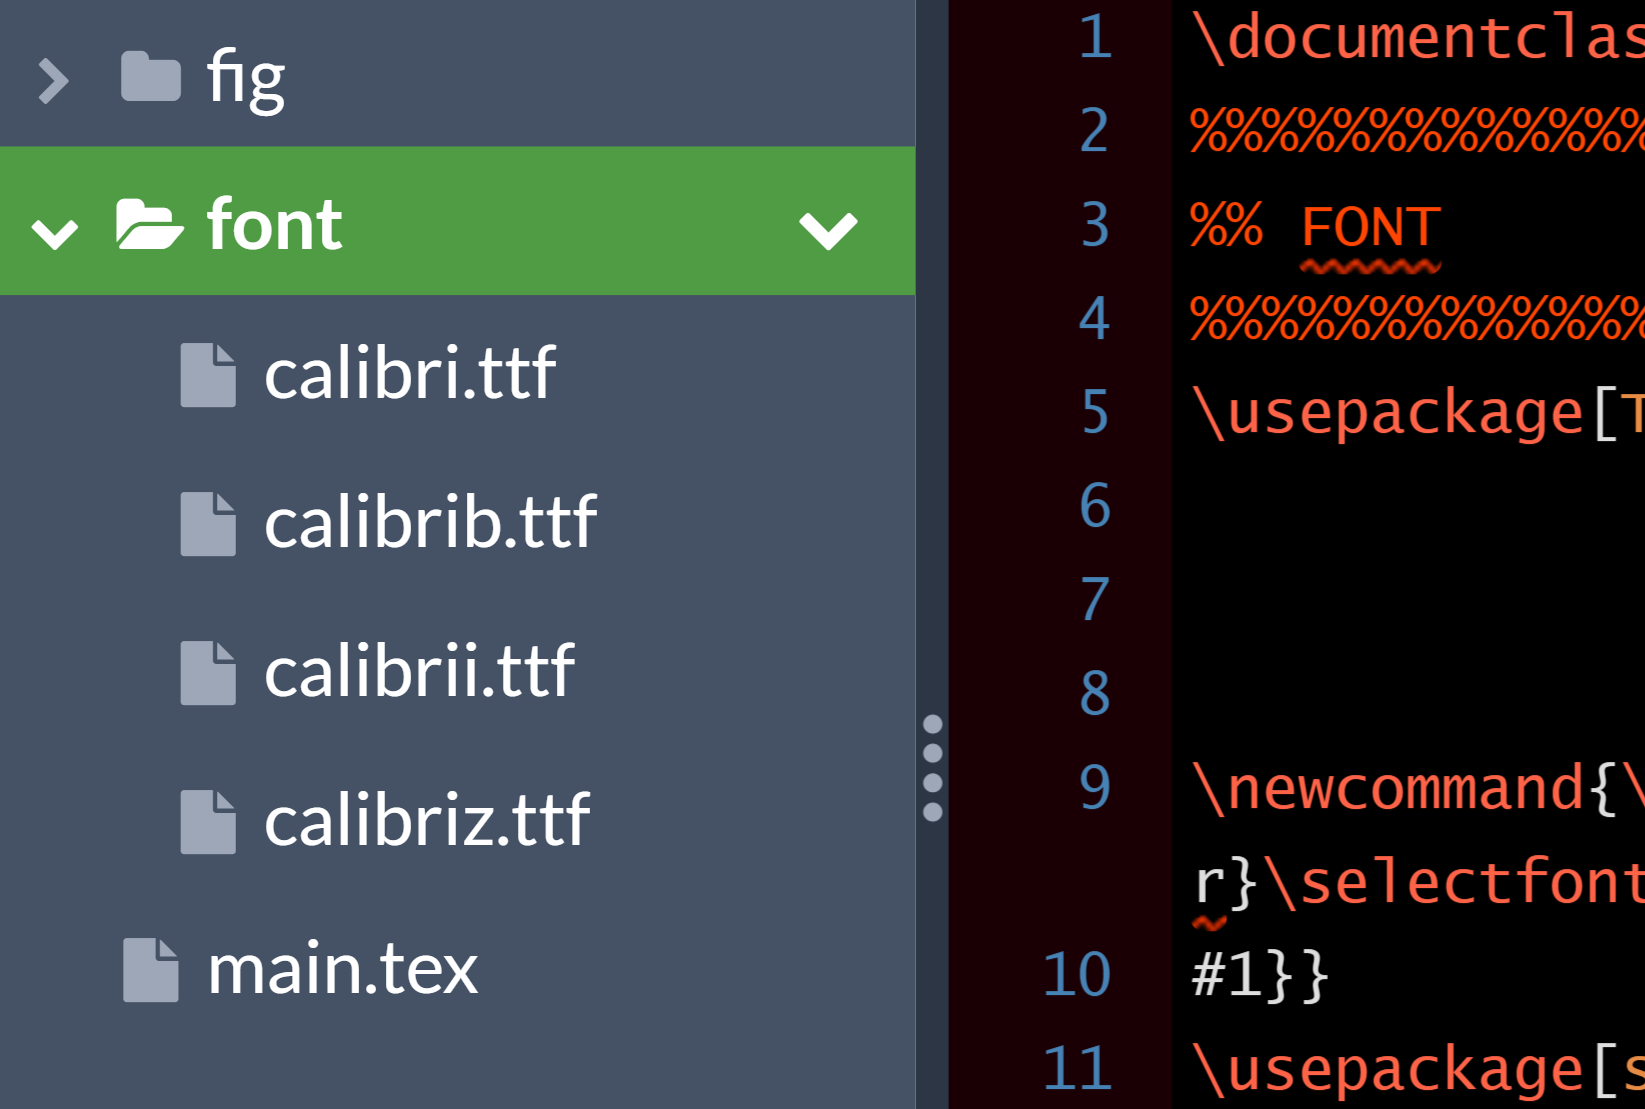
\includegraphics[width=8cm]{fig/fontpath.png}
    \caption{Carpeta de trabajo para el código \ref{cod:ttfexample} }
    \label{fig:ttfexample}
\end{figure}

\subsection{Fuentes recomendadas por el autor}
Ver tabla \ref{tab:recommendedfonts}.

\begin{table}[htb!] 

\begin{tabular}{llll}
 {\bf Fuente}&{\bf Paquete}  & \textbi{Font code} & {\bf Ejemplo}  \\\hline\vspace{.2cm}
 Concrete Roman & \vbfont{concrete}  & \vbfontbf{ccr}  & {\large \dofont{ccr}}  \\\hline\vspace{.2cm}
 Utopia & \vbfont{mathdesign} & \vbfontbf{mdput} & {\large \dofont{mdput}} \\\hline
 Helvetica &\vbfont{helvet}  & \vbfontbf{phv}  & {\large \dofont{phv}}  \\ \hline\vspace{.1cm}
 Comic Sans MS & \vbfont{fontspec} & \vbfontbf{comic} & {\cmcsans \large \lazyfox} \\ \hline \vspace{.2cm}

 &  &  & 
\end{tabular}
\caption{Para este documento se uso Utopia del paquete \vbfont{mathdesign}}
\label{tab:recommendedfonts}
\end{table}

\end{document}

%COSAS A AGREGAR


Cosas a agregar
\begin{itemize}
    \item \verb|\input{}|
    \item Array
    \item extsizes (canastory)
    \item macros
    \item footnotes no numericas-> agregar a la parte de footnotes
    \item vale la pena meter \( \) ?
    \item Title para doble columna tipo resumen MCI
    \item \linebreak \\, \par differences
\end{itemize}

Arrays = tablas pero con $ $ metidos automáticamente

comandos para ahorrar espacio
vspace



Corregir que Liantze hizo el catalogo para *fontspec*, no?



\ref{eq:miGranEcuacion}. agregar subseccion mostrando referencia \ref{eq:miGranEcuacion} Y mostrar \eqref{cod:firstblood}